\documentclass[12pt]{article}

\usepackage[a4paper, margin=2.5cm]{geometry}

\usepackage{amsthm}
\usepackage{circuitikz}
\usepackage{graphicx}
\usepackage{fontspec}
\usepackage{polyglossia}
\usepackage{hyperref}
\usepackage{pgfplots}
\pgfplotsset{compat=1.18}

\pgfplotsset{
  opamp plot/.style={
    width=7cm, height=6.5cm,
    axis lines=middle,
    axis line style={black, thick, -{Stealth[length=2.5mm]}},
    xmin=-1.2, xmax=1.2,
    ymin=-13,  ymax=13,
    xtick={-1,-0.5,0.5,1},
    ytick={-10,-5,5,10},
    minor tick num=0,
    grid=major,
    major grid style={gray!25, very thin},
    tick style={black},
    tick label style={font=\small},
    xlabel={$V_{in}\,[\mathrm{V}]$},
    ylabel={$V_{out}\,[\mathrm{V}]$},
    xlabel style={at={(current axis.right of origin)}, anchor=west},
    ylabel style={at={(current axis.above origin)}, anchor=south},
    title style={font=\bfseries, yshift=1.5ex},
    every axis plot/.append style={black, very thick, no markers},
  }
}


\setmainlanguage{serbian}
\setdefaultlanguage[script=Latin]{serbian}
\setmainfont{Times New Roman}

\title{Vežbe 2 - Operacioni pojačavač u otvorenoj i zatvorenoj sprezi}
\date{}
\author{}
\tikzset{
    my voltage/.style={
        circuitikz/voltage/distance from node=0.75,
    }
}

\begin{document}

\maketitle

\section{Operacioni pojačavač}

{Operacioni pojačavac je aktivna provodnička komponenta koja
pojačava razliku potencijala na svojim ulazima. Aktivna je komponenta
zato što za svoj rad zahteva spoljašnje napajanje, čime se omogućava
da izlazni signal ima veću snagu od ulaznog signala.
Izgled operacionog pojačavača je prikazan na slici \ref{fig:opamp}.}

\begin{figure}[ht]
    \centering
    \begin{circuitikz}[american]
        \begin{scope}
            \ctikzset{tripoles/op amp/width=2.5,   % default 2.5
                    tripoles/op amp/height=2}    % default 2
            \node[op amp] (OA) at (0,0) {};
        \end{scope}
        \draw
            (OA.+) -- ++(-1,0) node[left]{$V^{+}$}
            (OA.-) -- ++(-1, 0) node[left]{$V^{-}$}
            (OA.out) -- ++(1,0) node[right]{$V_{out}$};

        \draw
            (OA.up) -- ++(0,1) node[above]{$+V_{cc}$};

        \draw
            (OA.down) -- ++(0,-1) node[below]{$-V_{cc}$};
    \end{circuitikz}
    \caption{Operacioni pojačavač}
    \label{fig:opamp}
\end{figure}

{Operacioni pojačavač ima dva naponska ulaza, jedan je invertujući $V^{-}$,
a drugi neinvertujući $V^{+}$ i jedan izlaz $V_{out}$. Takođe ima dva priključka
za napajanje $+V_{cc}$ i $-V_{cc}$. Operacioni pojačavač na svom izlazu
$V_{out}$ daje pojačanu razliku potencijala na ulazima $V^{+}$ i $V^{-}$.
Ovo je dato sledećim izrazom}

\begin{equation}
    V_{out} = A_{o} \cdot (V^{+} - V^{-}).
\end{equation}

{$A_{o}$ predstavlja pojačanje operacionog pojačavača
u otvorenoj sprezi. Njegova vrednost zavisi od karakteristika
i specifikacije konkretnog operacionog pojačavača, obično je reda veličine $10^5$ do $10^6$. Vrednosti na izlazu operacionog pojačavača su ograničene napajanjem, tako da se uvek kreću između $+V_{cc}$ i $-V_{cc}$. Iz ovog zaključka može se izvesti izraz za maksimalnu vrednost ulaza operacionog pojačavača}

\begin{equation}
    -V_{cc} \le V_{out} \le +V_{cc},
\end{equation}

{odnosno zato što je $V_{out} = A_o V_{in}$}

\begin{equation}
    \frac{-V_{cc}}{A_o} \le V_{in} \le \frac{+V_{cc}}{A_o}.
\end{equation}

{Demonstracija u \href{https://www.desmos.com/calculator/83gqbywenh}{Desmos}-u}

\pagebreak
\subsection{Karakteristike idealnog operacionog pojačavača}

{Shema idealnog operacionog pojačavača data je na slici \ref{fig:opamp_ideal}.}

\begin{figure}[ht]
    \centering
    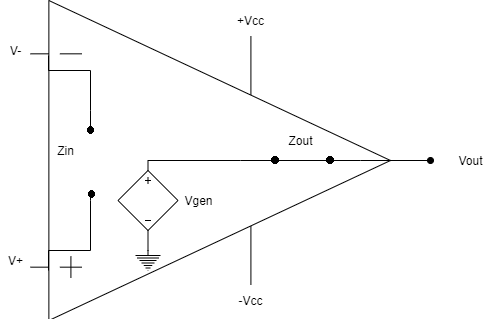
\includegraphics[width=0.6\textwidth]{opamp_ideal.png}
    \caption{Shema idealnog operacionog pojačavača.}
    \label{fig:opamp_ideal}
\end{figure}

{Na osnovu slike može se zaključiti da idealni operacioni pojačavač
ima sledeće karakteristike:}

\begin{enumerate}
    \item {$A_{o} = \infty$} - operacioni pojačavač u otvorenoj sprezi
    ima beskonačno veliko pojačanje, što znači da će i za najmanju razliku potencijala 
    na ulazu imati beskonačno veliki izlazni napon.
    \item {$Z_{in} = \infty$} - operacioni pojačavač ima beskonačno veliku ulaznu impedansu, što znači da ne teče struja kroz ulazne priključke operacionog pojačavača.
    \item {$Z_{out} = 0$} - operacioni pojačavač ima nultu ulaznu impedansu, što znači da se ponaša kao idealni naponski izvor (ne opterećuje kolo na bilo koji način).
    \item {Karakteristike rada operacionog pojačavača ne zavise od frekvencije ulaznog signala}
\end{enumerate}

{Ovakva izvedba operacionog pojačavača predstavlja samo idealizovan matematički
model i kao takav nije ga moguće realizovati u praksi. Već se on može
posmatrati kao nešto čemu inženjeri teže pri dizajniranju operacionih pojačavača.}

\section{Operacioni pojačavač u zatvorenoj sprezi}

{Problem kod izvedbe operacionog pojačavača u otvorenoj sprezi je u tome što se izlazni napon $V_{out}$ veoma lako može dovesti u stanje saturacije. Zbog veoma velikog pojačanja $A_{o}$, čak i izuzetno male vrednosti diferencijalnog napona na ulazu mogu dovesti do maksimalne vrednosti izlaznog napona. Zbog toga je operacioni pojačavač u otvorenoj sprezi praktično neupotrebljiv za potrebe linearnog pojačanja signala. Na primer, ako bi diferencijalni napon na ulazu iznosio $1,\mu\mathrm{V}$, na izlazu bi se dobila vrednost od $100,\mathrm{V}$. Međutim, isti izlazni napon bi se dobio i za ulazne napone od $10,\mu\mathrm{V}$, $100,\mu\mathrm{V}$, $1,\mathrm{mV}$ itd. Na taj način praktično nije moguće razlikovati različite vrednosti ulaznog signala, jer sve one rezultuju istom vrednošću izlaznog signala, odnosno ne dobijamo linearno mapiranje ulaznog signala na izlazni signal.}

{Zbog toga se operacioni pojačavači u praksi koriste u zatvorenoj sprezi, pri čemu se deo izlaznog signala vraća na ulaz operacionog pojačavača. Na taj način se postiže rad operacionog pojačavača u linearnom režimu, odnosno omogućava se da se izlazni signal $V_{out}$ menja u skladu sa ulaznim signalom $V_{in}$, pri čemu se izbegava saturacija. Ovime se dobija linearno mapiranje ulaznog signala na izlazni.}

{Postoje dve izvedbe operacionog pojačavača u zatvorenoj sprezi koje se najčešće koriste, a to su: neinvertujući i invertujući operacioni pojačavač.}

\subsection{Neinvertujući operacioni pojačavač}

\begin{figure}[ht]
    \centering
    \begin{circuitikz}[american]
        \begin{scope}
            \ctikzset{tripoles/op amp/width=2.5,   % default 2.5
                    tripoles/op amp/height=2}    % default 2
            \node[op amp] (OA) at (0,0) {};
        \end{scope}
        \draw
            (OA.+) -- ++(-2,0) to [V, l_=$V_{in}$] ++(0,-1) node[ground] {}
            (OA.-) to [R, l_=$R_1$] ++(-4, 0) node[ground] {}
            (OA.out) -- ++(1,0) node[right]{$V_{out}$};

        \draw
            (OA.up) -- ++(0,1) node[above]{$+V_{cc}$};

        \draw
            (OA.down) -- ++(0,-1) node[below]{$-V_{cc}$};
        
        \coordinate (topV_minus) at ($(OA.-) + (0, 2.5)$);
        \coordinate (startarrow) at ($(OA.-) + (-1.25, 0)$);

        \draw[->]
            (startarrow) -- ++(1,0) node[midway, above] {$I_1$};

        \draw[->]
            (topV_minus) -- ++(1,0) node[midway, above] {$I_2$};

        \node[circ] at (OA.-) {};
        \node[below] at (OA.-) {$V^-$};
        \node[circ] at (OA.+) {};
        \node[below] at (OA.+) {$V^+$};
        \node[circ] at (OA.out) {};

        \draw
            (OA.-) -- (topV_minus) to [R, l=$R_2$] ++(3.5,0) -- (OA.out);

        
    \end{circuitikz}
    \caption{Neinvertujući operacioni pojačavač}
    \label{fig:opamp_noninverting}
\end{figure}

{U konfiguraciji neinvertujećeg operacionog pojačavača ulazni signal $V_{in}$ povezan je na neinvertujući ulaz $V^+$ operacionog pojačavača, a invertujući ulaz se preko otpornika $R_1$ dovodi na masu. Pod pretpostavkom da se radi o idealnom operacionom pojačavaču važi da je}

\begin{equation}
    V^- = V^+ = V_{in}.
\end{equation}

{Budući da je ulazna impedansa idealnog operacionog pojačavača beskonačna, kroz njegove ulazne priključke ne teče struja. Zbog toga su struje kroz otpornike $R_1$ i $R_2$ jednake, pa važi}

\begin{equation}
    I_1 = \frac{V^- - 0}{R_1} \quad i \quad I_2 = \frac{V_{out} - V^-}{R_2},
\end{equation}

{odnosno}

\begin{equation}
    I = \frac{V^- - 0}{R_1} = \frac{V_{out} - V^-}{R_2}.
    \label{eq:opamp_noninv}
\end{equation}

{Nakon izjednačavanja jednačina u izrazu \ref{eq:opamp_noninv} dobija se izraz za zavisnost izlaznog napona operacionog pojačavača od ulaznog napona}

\begin{equation}
    V_{out} = (1 + \frac{R_2}{R_1})V_{in},
\end{equation}

{gde je izraz $1 + \frac{R_2}{R_1}$ zapravo pojačanje operacionog pojačavača, odnosno}

\begin{equation}
    A_o = 1 + \frac{R_2}{R_1}.
\end{equation}

{Za razliku od otvorene sprege, gde je pojačanje određeno karakteristikama samog operacionog pojačavača, u konfiguraciji sa negativnom povratnom spregom pojačanje je određeno vrednostima otpornika $R_1$ i $R_2$.}

\subsection{Invertujući operacioni pojačavač}

\begin{figure}[ht]
    \centering
    \begin{circuitikz}[american]
        \begin{scope}
            \ctikzset{tripoles/op amp/width=2.5,   % default 2.5
                    tripoles/op amp/height=2}    % default 2
            \node[op amp] (OA) at (0,0) {};
        \end{scope}
        \draw
            (OA.+) -- ++(-2,0) node[ground] {}
            (OA.-) to [R, l_=$R_1$] ++(-4, 0) to [V, l_=$V_{in}$] ++(0,-1.4) node[ground] {}
            (OA.out) -- ++(1,0) node[right]{$V_{out}$};

        \draw
            (OA.up) -- ++(0,1) node[above]{$+V_{cc}$};

        \draw
            (OA.down) -- ++(0,-1) node[below]{$-V_{cc}$};
        
        \coordinate (topV_minus) at ($(OA.-) + (0, 2.5)$);
        \coordinate (startarrow) at ($(OA.-) + (-1.25, 0)$);

        \draw[->]
            (startarrow) -- ++(1,0) node[midway, above] {$I_1$};

        \draw[->]
            (topV_minus) -- ++(1,0) node[midway, above] {$I_2$};

        \node[circ] at (OA.-) {};
        \node[below] at (OA.-) {$V^-$};
        \node[circ] at (OA.+) {};
        \node[below] at (OA.+) {$V^+$};
        \node[circ] at (OA.out) {};

        \draw
            (OA.-) -- (topV_minus) to [R, l=$R_2$] ++(3.5,0) -- (OA.out);

        
    \end{circuitikz}
    \caption{Invertujući operacioni pojačavač}
    \label{fig:opamp_inverting}
\end{figure}

{U ovoj konfiguraciji operacionog pojačavača se neinvertujući ulaz $V^+$ povezuje na masu, a na invertujući ulaz je povezano ulazno napajanje $V_{in}$ preko otpornika $R_1$. Pod pretpostavkom da se radi o idealnom operacionom pojačavaču može da se zaključi da su tačke $V^-$ i $V^+$ na istom potencijalu, odnosno da je $V^-$ povezan na virtuelnu masu preko $V^+$ i važi}

\begin{equation}
    V^- = V^+ = 0
\end{equation}

{Kao i kod izvedbe neinvertujućeg operacionog pojačavača i ovde je izraz za struju u kolu}

\begin{equation}
    I_1 = \frac{V_{in} - 0}{R_1} \quad i \quad I_2 = \frac{0 - V_{out}}{R_2},
\end{equation}

{odnosno}

\begin{equation}
    I = \frac{V_{in} - 0}{R_1} = \frac{0 - V_{out}}{R_2}.
\end{equation}

{I odavde može da se zaključi da je izraz koji određuje zavisnost izlaza od ulaza jednak}

\begin{equation}
    V_{out} = -\frac{R_2}{R_1} \cdot V_{in}.
\end{equation}

{Treba primetiti da se u ovoj izvedbi operacionog pojačavača ulazni signal invertuje i u zavisnosti od vrednosti otpornika $R_1$ i $R_2$, signal takođe može biti pojačan, oslabljen ili samo biti invertovan.}
\section{Zadaci}

\newtheorem{zadatak}{Zadatak}

\begin{zadatak}
    Odrediti izraz za signal na ulazu operacionog pojačavača u otvorenoj sprezi kako bi se na izlazu u potpunosti preneo ulazni signal ako je
    $A_o = 1\,M\,\frac{V}{V}$ i $\pm V_{cc} = \pm 10\,V$.

    \begin{enumerate}
        \item[a)] Prikazati odnos ulaza i izlaza za dati operacioni pojačavač.
        
        \item[b)] Prikazati izlaz operacionog pojačavača za proizvoljni ulazni signal.
    \end{enumerate}
    Razmisliti: Šta ako se ulazni signal dovede na invertujući ulaz operacionog pojačavača, a šta ako se dovede na neinvertujući? Šta ako se dovedu 2 ulaza na invertujući i neinvertujući ulaz operacionog pojačavača?
\end{zadatak}

\begin{zadatak}
    Odrediti signal na izlazu neinvertujućeg operacionog pojačavača i odnos ulaza i izlaza operacionog pojačavača ako su otpornosti $R_1 = 10 \,k\Omega$ i $R_2 = 50 \,k\Omega$, a napon napajanja $\pm V_{cc} = \pm 10\,V$. Na ulaz operacionog pojačavača se dovode signali:
    \begin{enumerate}
        \item[a)] $1V\sin{(100 \pi t)}$ i
        
        \item[b)] $3V\sin{(100 \pi t)}$.
    \end{enumerate}
    Prikazati simulaciju u trajanju od 0.01 sekunde.
\end{zadatak}

\begin{zadatak}
    Odrediti signal na izlazu invertujućeg operacionog pojačavača i odnos ulaza i izlaza operacionog pojačavača ako su otpornosti $R_1 = 10 \,k\Omega$ i $R_2 = 50 \,k\Omega$, a napon napajanja $\pm V_{cc} = \pm 10\,V$. Na ulaz operacionog pojačavača se dovode signali:
    \begin{enumerate}
        \item[a)] $1V\sin{(4 \pi t)}$ i
        
        \item[b)] $3V\sin{(4 \pi t)}$.
    \end{enumerate}
    Prikazati simulaciju u trajanju od 1 sekunde.
\end{zadatak}

\pagebreak
\section{Zadaci za vežbu}

\begin{zadatak}
    Odrediti izraz za izlaz iz operacionog pojačavača $V_{out}$ sa slike \ref{fig:opamp_zad1}.

    \begin{figure}[ht]
    \centering
    \begin{circuitikz}[american]
        \begin{scope}
            \ctikzset{tripoles/op amp/width=2.5,   % default 2.5
                    tripoles/op amp/height=2}    % default 2
            \node[op amp] (OA) at (0,0) {};
        \end{scope}
        \draw
            (OA.+) -- ++(-2,0) to [V, l_=$V_{2}$] ++(0,-1) node[ground] {}
            (OA.-) to [R, l_=$R_1$] ++(-4, 0) to [V, l_=$V_1$] ++(0,-2.4) node[ground] {}
            (OA.out) -- ++(1,0) node[right]{$V_{out}$};

        \draw
            (OA.up) -- ++(0,1) node[above]{$+V_{cc}$};

        \draw
            (OA.down) -- ++(0,-1) node[below]{$-V_{cc}$};
        
        \coordinate (topV_minus) at ($(OA.-) + (0, 2.5)$);
        \coordinate (startarrow) at ($(OA.-) + (-1.25, 0)$);

        \draw[->]
            (startarrow) -- ++(1,0) node[midway, above] {$I_1$};

        \draw[->]
            (topV_minus) -- ++(1,0) node[midway, above] {$I_2$};

        \node[circ] at (OA.-) {};
        \node[below] at (OA.-) {$V^-$};
        \node[circ] at (OA.+) {};
        \node[below] at (OA.+) {$V^+$};
        \node[circ] at (OA.out) {};

        \draw
            (OA.-) -- (topV_minus) to [R, l=$R_2$] ++(3.5,0) -- (OA.out);

        
    \end{circuitikz}
    \caption{Operacioni pojačavač sa dva ulaza}
    \label{fig:opamp_zad1}
    \end{figure}

    Razmisliti: Kako različiti odnosi ulaza $V_1$ i $V_2$ utiču na izlaz operacionog pojačavača?
\end{zadatak}

\begin{zadatak}
    Odrediti izraz za izlaz iz sabirača sa slike \ref{fig:opamp_zad2}.

    \begin{figure}[ht]
    \centering
    \begin{circuitikz}[american]
        \begin{scope}
            \ctikzset{tripoles/op amp/width=2.5,   % default 2.5
                    tripoles/op amp/height=2}    % default 2
            \node[op amp] (OA) at (0,0) {};
        \end{scope}

        \coordinate (crossroad) at ($(OA.+) + (-2,-0.5)$);

        \draw
            (OA.+) -- ++(-2,0) -- ++(0, -0.5) to [R, l=$R$] ++(-2, 0) to [V, l=$V_1$] ++ (-1,0) node[ground] {}
            (OA.-) to [R, l_=$R_1$] ++(-4, 0) node[ground] {}
            (OA.out) -- ++(1,0) node[right]{$V_{out}$};
        \draw
            (crossroad) -- ++(0,-2) to [R, l=$R$] ++(-2, 0) to [V, l=$V_2$] ++ (-1,0) node[ground] {};
        
        \draw
            (OA.up) -- ++(0,1) node[above]{$+V_{cc}$};

        \draw
            (OA.down) -- ++(0,-1) node[below]{$-V_{cc}$};
        
        \coordinate (topV_minus) at ($(OA.-) + (0, 2.5)$);
        \coordinate (startarrow) at ($(OA.-) + (-1.25, 0)$);

        \draw[->]
            (startarrow) -- ++(1,0) node[midway, above] {$I_1$};

        \draw[->]
            (topV_minus) -- ++(1,0) node[midway, above] {$I_2$};

        \node[circ] at (OA.-) {};
        \node[below] at (OA.-) {$V^-$};
        \node[circ] at (OA.+) {};
        \node[below] at (OA.+) {$V^+$};
        \node[circ] at (OA.out) {};

        \draw
            (OA.-) -- (topV_minus) to [R, l=$R_2$] ++(3.5,0) -- (OA.out);

        
    \end{circuitikz}
    \caption{Sabirač}
    \label{fig:opamp_zad2}
    \end{figure}
    Razmisliti: Kako bi izgledao izlaz operacionog pojačavača za sličnu konfiguraciju na invertujućem ulazu?
\end{zadatak}

\end{document}